\documentclass[a4paper, 12pt]{article}
\usepackage[a4paper,top=1.5cm, bottom=1.5cm, left=1cm, right=1cm]{geometry}
\usepackage{cmap}					% поиск в PDF
\usepackage{mathtext} 				% русские буквы в формулах
\usepackage[T2A]{fontenc}			% кодировка
\usepackage[utf8]{inputenc}			% кодировка исходного текста
\usepackage[english,russian]{babel}	% локализация и переносы

\usepackage{amsmath}
\usepackage{indentfirst}
\usepackage{longtable}
\usepackage{graphicx}
\usepackage{array}

\usepackage{wrapfig}
\usepackage{siunitx} % Required for alignment
\usepackage{subfigure}
\usepackage{multirow}
\usepackage{rotating}
\usepackage{caption}

\graphicspath{{.}}


\title{\begin{center}Лабораторная работа №2.1.4\end{center}
Определение теплоемкости твердых тел}
\author{Рожков А. В. \\ Преподаватель Яворский В. А.}
\date{\today}

\begin{document}
    \pagenumbering{gobble}
    \maketitle
    \newpage
    \pagenumbering{arabic}

    \textbf{Цель работы:} 1. прямое измерение кривых нагревания $T_{heat}(t)$ и охлаждения $T_{cool}(T)$ пустого калориметра и системы «калориметр + твердое тело»; 2. определение коэффициента теплоотдачи стенок калориметра; 3. определение теплоемкости пустого калориметра и удельной теплоемкости твердого тела

	\textbf{В работе используются:} калориметр с нагревателем и термометром сопротивления; универсальный вольтметр В7-78/3 в режиме омметра ($\sigma_{T} = 0.05~K$), измеритель температуры - термопара K-типа совместно с универсальным вольтметром В7-78/2 ($\sigma_{T_{комн}} = 0.1~K$), источник питания GPS-72303, универсальные вольтметры В7-78/3 (в режиме амперметра) ($\sigma_I = 0.01~A$) и KEITHLEY (в режиме вольтметра) ($\sigma_U = 0.1~В$) для измерения мощности нагревателя, компьютерная программа АКИП для сопряжения персонального компьютера и универсальных вольтметров В7-78/2 и В7-78/3 ($\sigma_t = 0.01~с$).

    \section{Теоретическая справка}

        В данной работе теплоемкость определяется по формуле
        \begin{equation}
            C = \frac{\Delta Q}{\Delta T},
            \label{eq:dQdT}
        \end{equation}
        где $\Delta Q$ -- количество тепла, подведенного к телу, и $\Delta T$ -- изменение температуры тела, произошедшее в результате подвода тепла.

        Температура внутри калориметра измеряется термометром сопротивления. В реальных условиях $\Delta Q \neq P \Delta t$, так как часть энергии уходит из калориметра благодаря теплопроводности его стенок. В результате количество тепла $\Delta Q = C \Delta T$, подведённое к системе "тело + калориметр" будет меньше на величину тепловых потерь:

        \begin{equation}
            C \Delta T = P \Delta t - \lambda(T - T_к) \Delta T
            \label{eq:C_Delta_T}
        \end{equation}
        где $\lambda$ - коэффициент теплоотдачи стенок калориметра, $T$ - температура тела и калориметра, $T_к$ - комнатная температура.

        Уравнение (\ref{eq:C_Delta_T}) является основной расчетной формулой работы. В дифференциальной форме для процессов нагревания и охлаждения ($P = 0$) соответственно оно имеет следующий вид:

        \begin{align}
            C dT &= P dt - \lambda \left[ T_{heat}(t) - T_к(t) \right] dt \label{eq:CdT} \\
            C dT &= - \lambda \left[ T_{cool}(t) - T_к(t) \right] dt \label{eq:CdT2}
        \end{align}
        где $P$ ‒ мощность нагревателя, $\lambda$ ‒ коэффициент теплоотдачи стенок калориметра, $t$ – время, измеряемое от момента включения нагревателя, $T_{heat}(t)$ ‒ температура тела в момент времени $t$ на кривой нагревания, $T_{cool}(t)$ ‒ температура тела в момент времени $t$ на кривой охлаждения, $T_к(t)$ ‒ температура окружающего калориметр воздуха (комнатная) в момент времени $t$, $dt$ ‒ время, в течение которого температура тела изменилась на $dT$

        \subsection{Экспериментальная установка}

            Установка состоит из калориметра с пенопластовой изоляцией, помещенного в ящик из многослойной клееной фанеры. Внутренние стенки калориметра выполненным из материала с высокой теплопроводностью. Надежность теплового контакта между телом и стенками обеспечивается их формой: они имеют вид усеченных конусов и плотно прилегают друг к другу.

            \begin{figure}[ht]
                \centering
                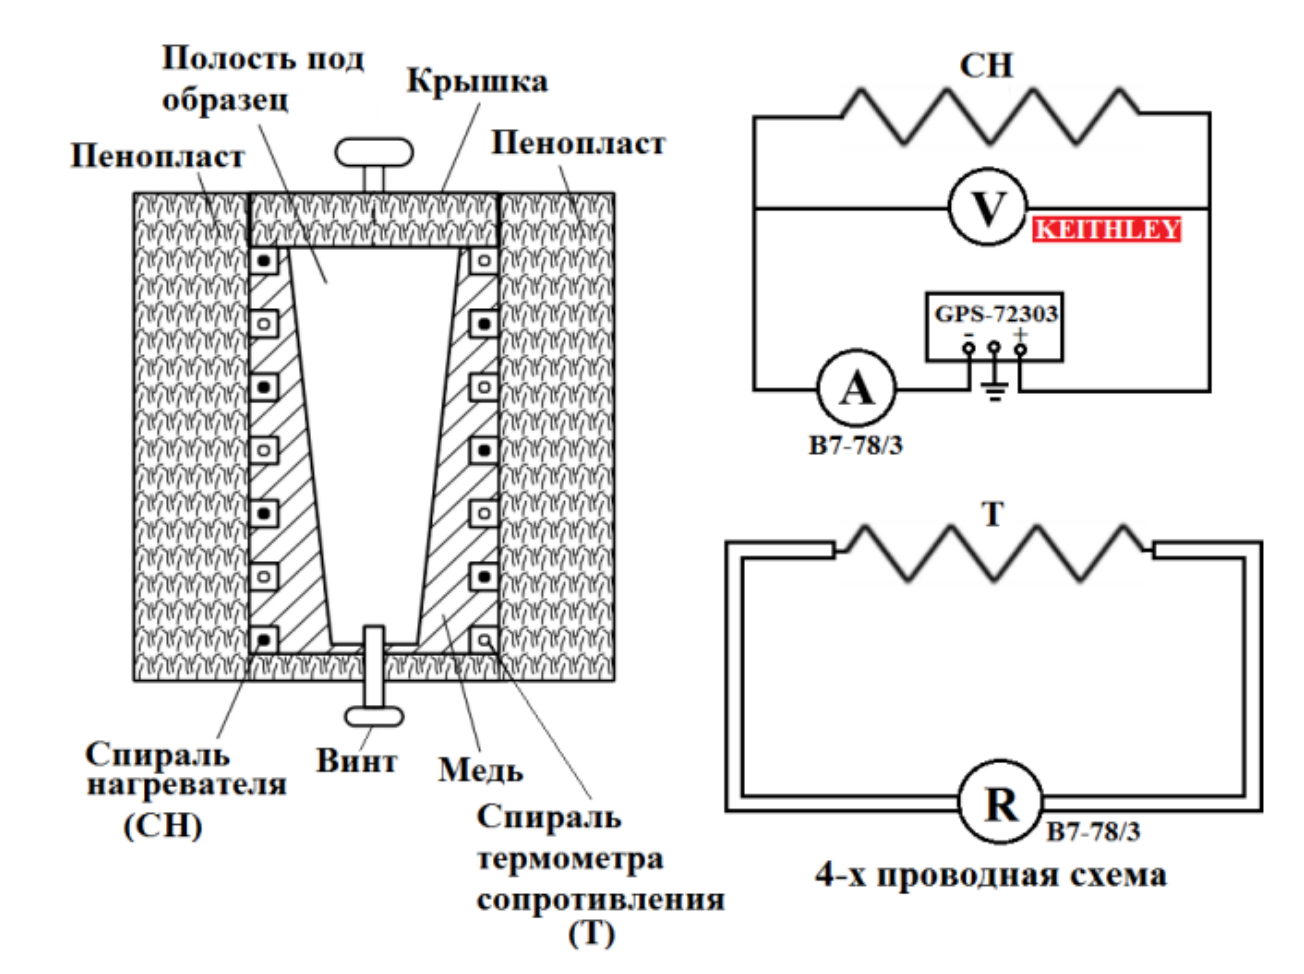
\includegraphics[width=0.8\textwidth]{img/calorimeter.png}
                \caption{Схема устройства калориметра}
                \label{fig:calorimeter}
            \end{figure}

            Экспериментально измеряемые данные:

                1. $R_{heat}(t)$ ‒ кривая зависимости термометра сопротивления от времени при нагревании калориметра с телом при P=const.

                2. $R_{cool}(t)$ ‒ кривая зависимости термометра сопротивления от времени при охлаждении калориметра с телом при $P = 0$ (нагреватель выключен!).

                3. $T_к(t)$ ‒ кривая зависимости комнатной температуры от времени

        \subsection{Методика эксперимента}

            Температура измеряется термометром сопротивления. Сопротивление проводника изменяется с температурой по закону

            \begin{equation}
                R_{T} = R_{273}(1 + \alpha (T - 273)),
                \label{RT}
            \end{equation}
            где $R_{T}$ -- сопротивление термометра про $T  ^{\circ}C$, $R_{0}$ -- его сопротивление при $0  ^{\circ}C$, $\alpha$ -- температурный коэффициент сопротивления.

            Выразим сопротивление $R_{273}$ через измеренное значение $R_{к}$ -- сопротивление термометра при комнатной температуре. Согласно (\ref{RT}), имеем

            \begin{equation}
                R_{273} = \frac{R_{к}}{1 + \alpha (T_к - 273)},
                \label{R273}
            \end{equation}

            Подставляя (\ref{R273}) в (\ref{RT}), найдём:

            \begin{equation}
                T(R_T) = 273 + \frac{R_T}{\alpha R_к} \left[ 1 + \alpha (T_к - 273) \right] - \frac{1}{\alpha}
                \label{T_R_T}
            \end{equation}

            Формула (\ref{T_R_T}) позволяет легко пересчитать кривые $R_{heat}(t)$, $R_{cool}(t)$ в кривые $T_{heat}(t)$, $T_{cool}(t)$. Входящий в формулу температурный коэффициент сопротивления меди равен $\alpha = 4.28*10^{-3} град^{-1}$.

            Из уравнения (\ref{eq:CdT2}) при $T_к(t) = T_к = const$:

            \begin{equation}
                C dT_{cool} = - \lambda \left[ T_{cool} - T_к \right] dt
                \label{C_dT_cool}
            \end{equation}

            Это дифференциальное уравнение с разделяющимися переменными $T_{cool}$ и $t$:

            \begin{equation}
                \frac{C dT_{cool}}{- \lambda \left[ T_{cool} - T_{к} \right]} = dt
                \label{eq:diff}
            \end{equation}

            После интегрирования в пределах от $t=0$ ($T_{cool} = T$) до произвольного момента времени $t$:

            \begin{equation}
                \frac{-C}{\lambda} ln \frac{T_{cool} - T_{к}}{T - T_к} = t
                \label{eq:diff_integral}
            \end{equation}

            Отсюда находим явную зависимость от времени:

            \begin{equation}
                T_{cool}(t) = (T - T_к) e^{\frac{- \lambda}{C} t} + T_к
                \label{T_cool_t}
            \end{equation}

            Уравнение (\ref{T_cool_t}) легко спрямляется в координатах ($ln \frac{T_{cool} - T_к}{T - T_к}$, $t$). Тангенс угла наклона данной прямой позволяет определить отношение искомых величин $\frac{\lambda}{C}$.

            Из уравнения (\ref{eq:CdT}) при $T_к(t) = T_к = const$:

            \begin{equation}
                C dT_{heat} = P dt - \lambda \left[ T_{heat} - T_к \right] dt
                \label{C_dT_heat}
            \end{equation}

            Это дифференциальное уравнение с разделяющимися переменными $T_{heat}$ и $t$:

            \begin{equation}
                \frac{C dT_{heat}}{P - \lambda \left[ T_{heat} - T_{к} \right]} = dt
                \label{eq:diff2}
            \end{equation}

            После интегрирования в пределах от $t = 0$ ($T_{heat} = T_к$) до произвольного момента времени $t$:

            \begin{equation}
                \frac{-C}{\lambda} ln \frac{P - \lambda (T_{heat} - T_{к})}{P} = t
                \label{eq:diff_integral2}
            \end{equation}

            Отсюда находим явную зависимость от времени:

            \begin{equation}
                T_{heat}(t) = \frac{P}{\lambda} (1 - e^{\frac{-\lambda}{C} t}) + T_к
                \label{T_heat_t}
            \end{equation}

            Уравнение (\ref{T_heat_t}) позволяет по найденному ранее из кривой охлаждения отношению $\frac{\lambda}{C}$ определить $\lambda$, а зная $\lambda$ и $\frac{\lambda}{C}$ легко найти искомую теплоемкость $С$.

            Метод измерений величин $С$ и $\lambda$ рассмотренный выше, дает хорошие результаты при стабильной комнатной температуре во время проведения эксперимента и является по своей сути интегральным. $С$ и $\lambda$ определяются из уравнений (\ref{T_cool_t}) и (\ref{T_heat_t}), которые следуют из уравнений (\ref{eq:CdT}) и (\ref{eq:CdT2}) после их интегрирования. При существенных колебаниях комнатной температуры ($\sim 2-3~^0C$) интегральные уравнения (\ref{T_cool_t}) и (\ref{T_heat_t}) могут привести к достаточно большой погрешности в определении величин $С$ и $\lambda$. В этом случае следует использовать дифференциальные методы, основанные на измерении величин $\left( \frac{dT}{dt} \right)_{heat}$ и $\left( \frac{dT}{dt} \right)_{cool}$ в окрестностях каких-либо «удобных» точек. К таким «удобным» точкам относится точка на кривой нагревания, при которой температура калориметра совпадает с комнатной. Действительно, дифференцируя уравнение (\ref{eq:CdT}) по времени при $T_{heat}(t) = T_к(t)$, получим простую и удобную формулу для определения теплоемкости $С$:

            \begin{equation}
                C = \frac{P}{(dT_{heat} / dt)_{T = T_к}}
                \label{eq:C}
            \end{equation}

            Она дает хорошие результаты, если ее применение никак не связано с моментом включения нагревателя. Причина проста: сразу после включения нагревателя в калориметре происходят переходные процессы формирования тепловых потоков, которые не описываются уравнением (\ref{eq:CdT}) и соответственно уравнением (\ref{eq:C}). Чтобы обойти данную трудность, перед включением нагревателя необходимо охладить калориметр до температуры на $\sim 2-5~^oC$ ниже комнатной. В этом случае при подходе к точке $T_{heat}(t) = T_к(t)$ все переходные процессы уже закончатся и уравнение (\ref{eq:C}) будет корректным.

            Другими «удобными» точками для определения $С$ и $\lambda$ являются точки при одной и той же температуре $T$ на кривых нагревания $T_{heat}(t)$ и охлаждения $T_{cool}(t)$ соответственно. Действительно продифференцируем уравнения (\ref{eq:CdT}) и (\ref{eq:CdT2}) по времени:

            \begin{align}
                C \left( \frac{dT}{dt} \right)_{heat} &= P - \lambda \left[ T_{heat}(t) - T_к(t) \right] \label{eq:C_diff_heat}\\
                C \left( \frac{dT}{dt} \right)_{cool} &= - \lambda \left[ T_{cool}(t) - T_к(t) \right] \label{eq:C_diff_cool}
            \end{align}

            Определим $A = \left( \frac{dT}{dt} \right)_{heat}$ и $B = \left( \frac{dT}{dt} \right)_{cool}$ при одной и той же температуре $T$ на кривых $_{heat}(t)$ и $T_{cool}(t)$ соответственно. Тогда с учетом введенных обозначений, решая систему уравнений (\ref{eq:C_diff_heat}) и (\ref{eq:C_diff_cool}), получим следующие выражения для $С$ и $\lambda$:

            \begin{align}
                \lambda &= \frac{P}{(T - T_{к2})(1 - \frac{A}{B}) + T_{к2} - T_{к1}} \label{eq:lambda}\\
                C &= \frac{P}{A - B + A \frac{T_{к1} - T_{к2}}{T - T_{к1}}} \label{eq:C2}
            \end{align}
            где $T_{к1}$ и $T_{к2}$ ‒ комнатная температура в моменты времени $t = t_1$ и $t = t_2$, когда $T_{heat}(t_1) = T_{cool}(t_2) = T$.

            В случае равенства комнатных температур, когда $T_{к1} = T_{к2} = T_к$ формулы (\ref{eq:lambda}) и (\ref{eq:C2}) упрощаются

            \begin{align}
                \lambda &= \frac{P}{(T - T_к)(1 - \frac{A}{B})} \label{eq:lambda_fin}\\
                C &= \frac{P}{A - B} \label{eq:C_fin}
            \end{align}

            \begin{figure}[ht]
                \centering
                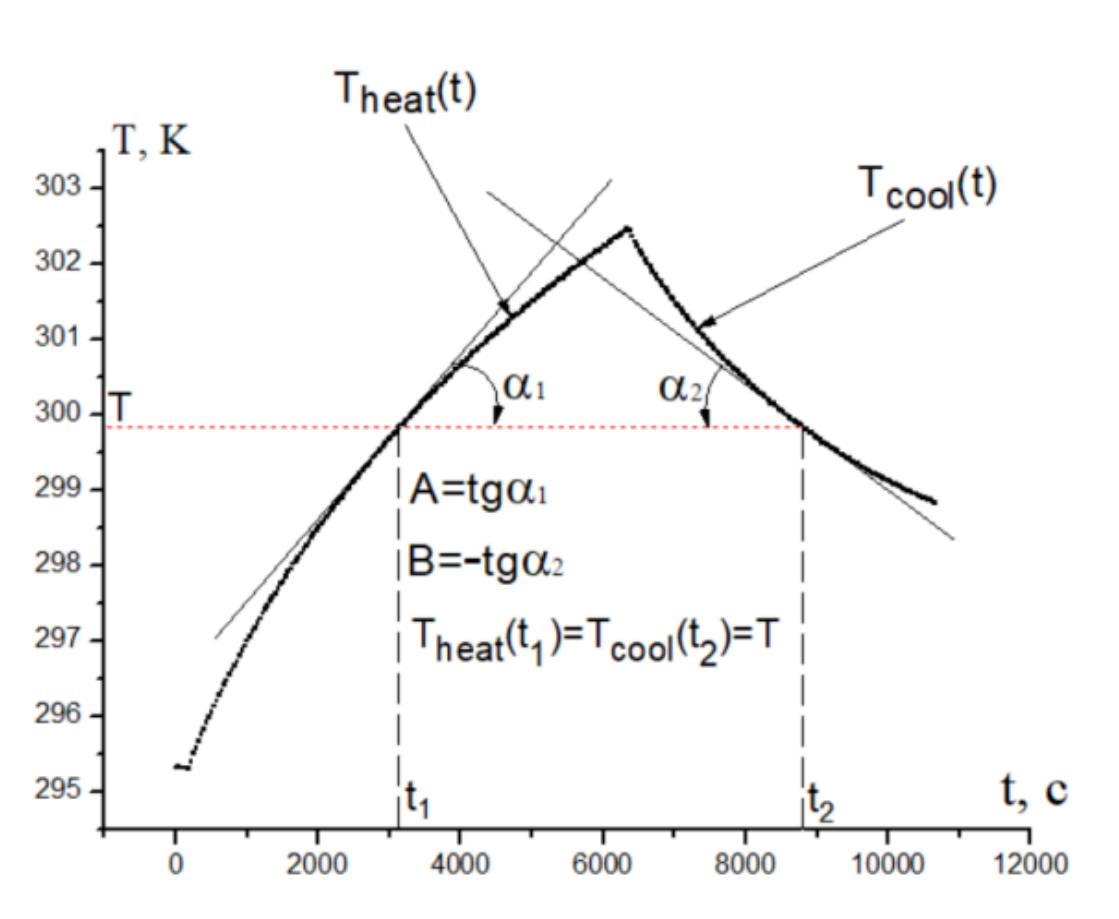
\includegraphics[width=0.6\textwidth]{img/diff_method.png}
            \end{figure}

            Следует иметь в виду, что определение величины $B$ на кривой охлаждения $T_{cool}(t)$ необходимо производить на участках кривой достаточно далеких от момента выключения нагревателя, после того как в калориметре закончатся переходные процессы «переполюсовки» тепловых потоков. Корректный интервал времени для определения В можно определить экспериментально из кривой $T_{cool}(t)$, спрямляя ее в координатах ($ln \frac{T_{cool} - T_к}{T - T_к}$, $t$) , после чего исключить из рассмотрения начальный нелинейный участок:

            \begin{figure}[ht]
                \centering
                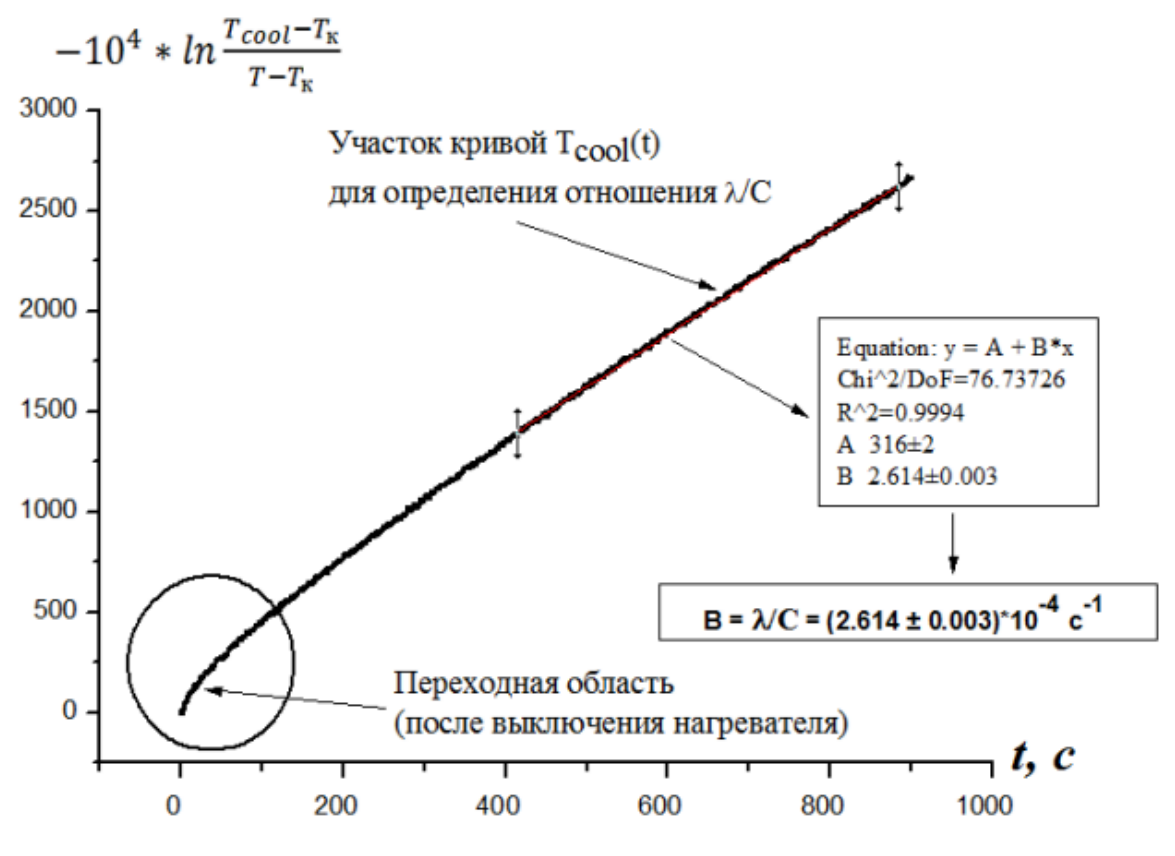
\includegraphics[width=0.6\textwidth]{img/not_lin_fragment.png}
            \end{figure}

    \section{Ход работы}

        \subsection{Проведение измерений}

            \subsubsection{Охлаждение калориметра}

                Вставляем в калориметр охлаждённый конус. Через 4 минуты после того, как температура в калориметре начинает медленно расти, вынимаем конус и ждём ещё 4 минуты. Калориметр охладился примерно на $5~^oC$.

            \subsubsection{Определение зависимости сопротивления терморезистора от времени при нагревании пустого калориметра}

                Включаем нагреватель, после того, как температура в калориметре превысила комнатную на $9~^oC$, отключаем цепь спирали нагревателя.

            \subsubsection{Определение зависимости сопротивления терморезистора от времени при охлаждении пустого калориметра}

                Продолжаем следить за изменением температуры калориметра. После того, как она уменьшилась на 2 градуса по сравнению с максимальной, приступаем к измерению теплоёмкости калориметра вместе с исследуемым телом.

            \subsubsection{Охлаждение калориметра}

                Снова охлаждаем калориметр до температуры на $5~^oC$ ниже комнатной. Вставляем в калориметр исследуемый образец и повторяем заново пункты 2-3.

            \subsubsection{Исследуемые образцы}

                Измерения проводим для образцов из алюминия и титана. Массы исследуемых образцов:

                \begin{align*}
                    m_{алюм} &= (294.1 \pm 0.5)~г & m_{титан} &= (293.2 \pm 0.5)~г
                \end{align*}

            \subsubsection{Окончание измерений}

                Останавливаем запись в программе. Сохраняем файлы с данным.

        \subsection{Обработка результатов измерений}

            \subsubsection{Сопоставление кривых с отметками времени в лабораторном журнале}

                По результатам измерений имеем общий график \ref{plot:all} (представлен в приложении).

                Сопоставим кривые с временными отметками:

                \begin{table}[!ht]
                    \centering
                    \begin{tabular}{|l|c|c|}
                        \hline

                        Событие & Начало, сек & Конец, сек\\ \hline
                        $T_{heat_1}(t)$ - нагрев пустого калориметра & 1000 & 2500\\ \hline
                        $T_{cool_1}(t)$ - охлаждение пустого калориметра & 2600 & 3700\\ \hline
                        $T_{heat_2}(t)$ - нагрев алюминия & 4800 & 6000\\ \hline
                        $T_{cool_2}(t)$ - охлаждение алюминия & 6300 & 6900\\ \hline
                        $T_{heat_3}(t)$ - нагрев титана & 7800 & 8600\\ \hline
                        $T_{cool_3}(t)$ - охлаждение титана & 8800 & 9300\\ \hline

                    \end{tabular}
                    \caption{Сопоставление кривых с отметками времени}
                    \label{tab:timetable}
                \end{table}

                Также видим, что комнатная температура менялась менее чем на $2~K$, значит мы можем использовать интегральный способ вычисления теплоёмкости.

            \subsubsection{Теплоёмкость пустого калориметра}

                Построим кривую $T_{cool}(t)$ в координатах ($ln \frac{T_{cool} - T_к}{T - T_к}$, $t$), где $T_к$ - среднее значение комнатной температуры за время измерения; $T$ - температура калориметра в начале кривой. соответствующий график \ref{plot:T_cool_1}:

                \begin{figure}[ht]
                    \centering
                    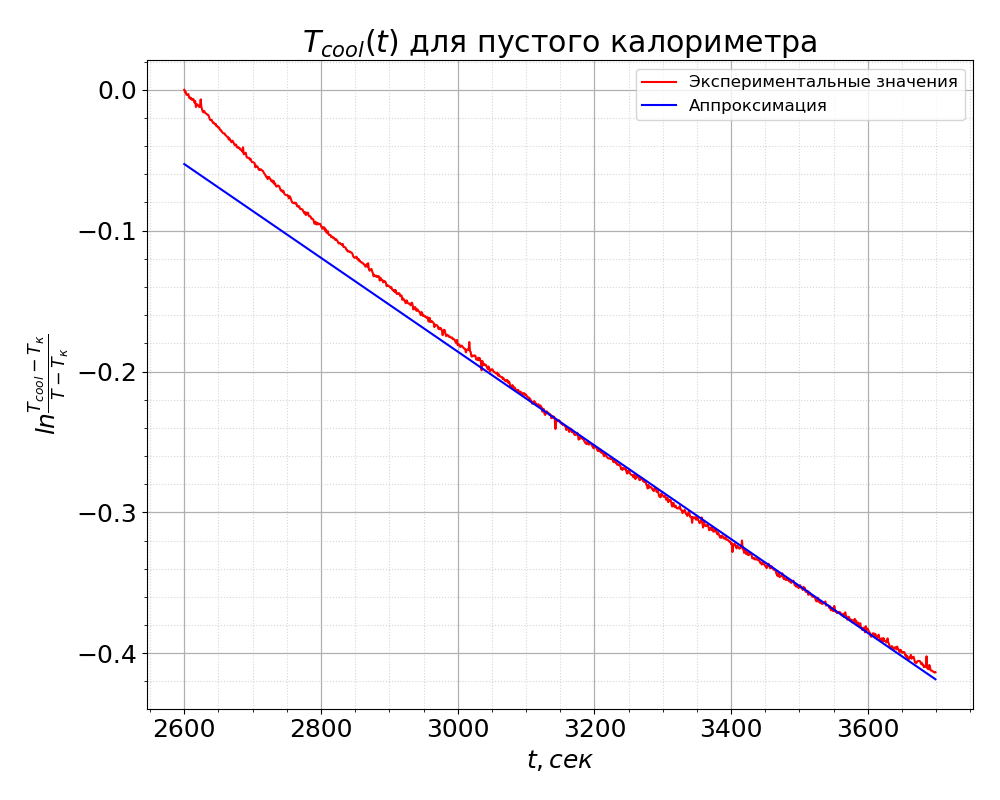
\includegraphics[width=0.6\textwidth]{img/graph_cool_1.png}
                    \caption{$T_{cool}(t)$ для пустого калориметра}
                    \label{plot:T_cool_1}
                \end{figure}

                Исключим начальный нелинейный участок и определим коэффициент угла наклона прямой по МНК. Из формулы (\ref{T_cool_t}) $\frac{\lambda}{C} = -k$.

                Приборная погрешность $\frac{\lambda}{C}$:

                \begin{equation*}
                    \sigma_{\frac{\lambda}{C}}^{приб} = \sqrt{ \left( \frac{1}{t} \frac{\lambda}{C} \right)^2 \sigma_t^2 + \left( \frac{1}{t} \frac{1}{T_{cool} - T_к} \right)^2 \sigma_{T_{cool}}^2 + \left( \frac{1}{t} \frac{T_{cool} - T}{(T_{cool} - T_к)(T - T_к)} \right)^2 \sigma_{T_к}^2 + \left( \frac{1}{t} \frac{1}{T - T_к} \right)^2 \sigma_T^2}
                \end{equation*}

                Итого результат с полной погрешностью:

                \begin{equation*}
                    \frac{\lambda}{C} = (33 \pm 2)*10^{-5}~с^{-1}
                \end{equation*}

                Из уравнения (\ref{T_heat_t}) ясно, что $\lambda$ можно найти по углу наклона прямой $T_{heat}\left(P(1 - e^{- \frac{\lambda}{C} t})\right)$. Из этой формулы $\lambda = \frac{1}{k}$. Приборная погрешность $\lambda$ и $C$:

                \begin{equation*}
                    \sigma_{\lambda}^{приб} = \sqrt{\left( \frac{\lambda}{P} \right)^2 \sigma_P^2 + \left( \frac{P t e^{-\frac{\lambda}{C} t}}{T_{heat} - T_к} \right)^2 \sigma_{\frac{\lambda}{C}}^2 + \left( \frac{P \frac{\lambda}{C} e^{-\frac{\lambda}{C} t}}{T_{heat} - T_к} \right)^2 \sigma_t^2 + \left( \frac{\lambda}{T_{heat} - T_к} \right)^2 \left( \sigma_{T_{heat}}^2 + \sigma_{T_к}^2 \right)}
                \end{equation*}
                \begin{equation*}
                    \sigma_C^{приб} = C \sqrt{\left( \frac{ \sigma_{\frac{\lambda}{P}}}{\frac{\lambda}{P}} \right)^2 + \left( \frac{\sigma_{\lambda}}{\lambda} \right)^2}
                \end{equation*}

                Итого результат с полной погрешностью:

                \begin{equation*}
                    \lambda = (0.24 \pm 0.02)~\frac{Дж}{К*с}
                \end{equation*}

                \begin{equation*}
                    C_{калориметр} = \lambda / \frac{\lambda}{C} = (0.73 \pm 0.07)~\frac{кДж}{К}
                \end{equation*}

            \subsubsection{Теплоёмкость алюминия}

                Аналогично предыдущему пункту определяем теплоёмкость алюминиевого образца вместе с калориметром, затем вычитаем теплоёмкость калориметра. соответствующий график \ref{plot:T_cool_2}:

                \begin{figure}[ht]
                    \centering
                    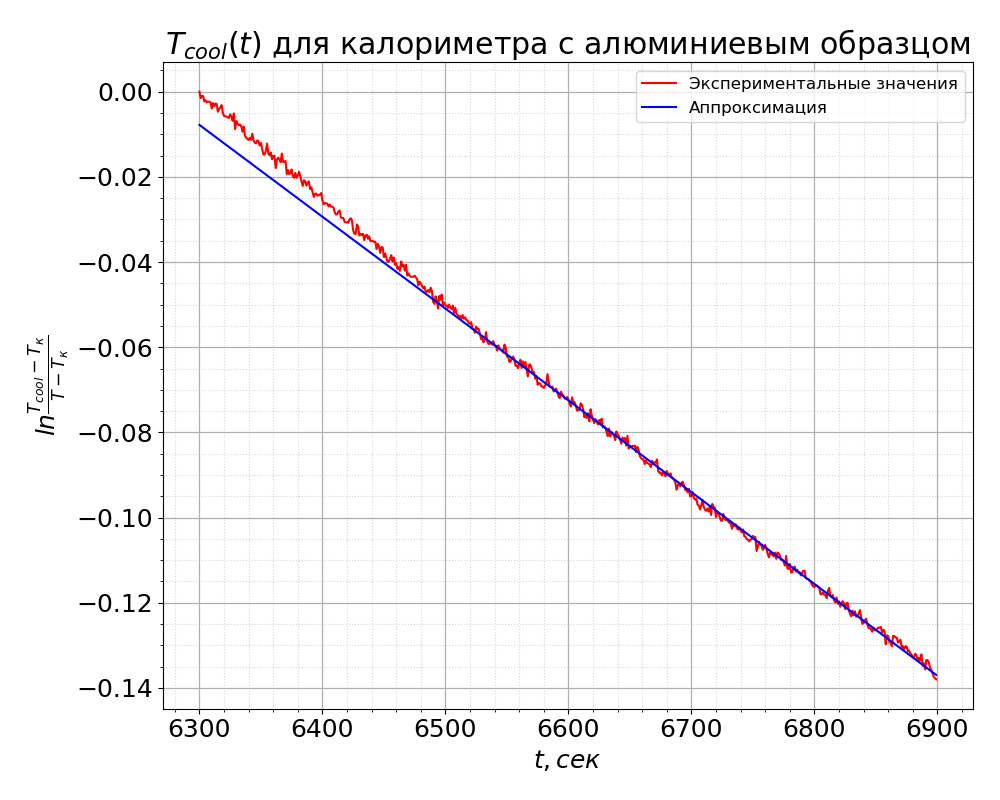
\includegraphics[width=0.6\textwidth]{img/graph_cool_2.png}
                    \caption{$T_{cool}(t)$ для калориметра с алюминиевым образцом}
                    \label{plot:T_cool_2}
                \end{figure}

                \begin{equation*}
                    \frac{\lambda}{C} = (22 \pm 4)*10^{-5}~с^{-1}
                \end{equation*}

                \begin{equation*}
                    \lambda = (0.21 \pm 0.04)~\frac{Дж}{К*с}
                \end{equation*}

                \begin{equation*}
                    C = \lambda / \frac{\lambda}{C} = (1.0 \pm 0.2)~\frac{кДж}{К}
                \end{equation*}

                \begin{equation*}
                    C_{алюм} = C - С_{калориметр} = (0.2 \pm 0.3)~\frac{кДж}{К}
                \end{equation*}

                \begin{equation*}
                    c_{алюм} = \frac{С_{алюм}}{m_{алюм}} = (0.8 \pm 0.9)~\frac{кДж}{кг*К}
                \end{equation*}

            \subsubsection{Теплоёмкость титана}

                Аналогично найдём все нужные значения для титана.

                \begin{figure}[ht]
                    \centering
                    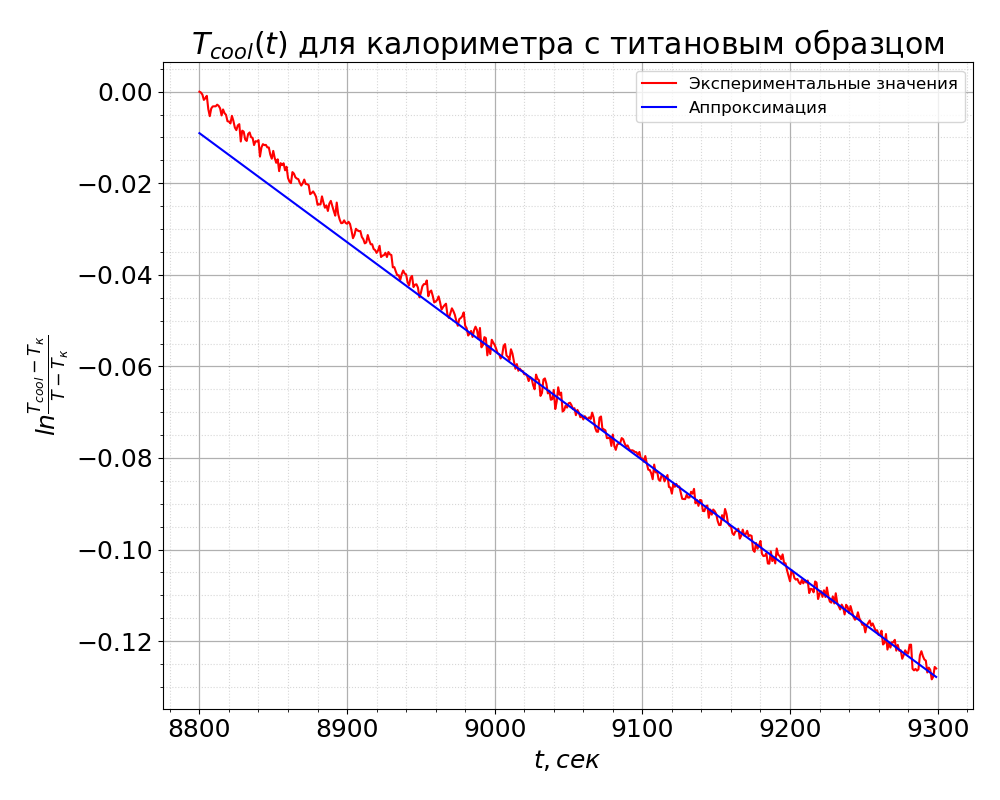
\includegraphics[width=0.6\textwidth]{img/graph_cool_3.png}
                    \caption{$T_{cool}(t)$ для калориметра с титановым образцом}
                    \label{plot:T_cool_3}
                \end{figure}

                \begin{equation*}
                    \frac{\lambda}{C} = (24 \pm 6)*10^{-5}~с^{-1}
                \end{equation*}

                \begin{equation*}
                    \lambda = (0.19 \pm 0.05)~\frac{Дж}{К*с}
                \end{equation*}

                \begin{equation*}
                    C = \lambda / \frac{\lambda}{C} = (0.8 \pm 0.3)~\frac{кДж}{К}
                \end{equation*}

                \begin{equation*}
                    C_{титан} = C - С_{калориметр} = (0.1 \pm 0.3)~\frac{кДж}{К}
                \end{equation*}

                \begin{equation*}
                    c_{титан} = \frac{С_{титан}}{m_{титан}} = (0.3 \pm 0.27)~\frac{кДж}{кг*К}
                \end{equation*}

            \subsubsection{Теплоёмкость пустого калориметра дифференциальным методом}

                Определим теплоёмкость пустого калориметра по формуле (\ref{eq:C}) в момент, когда температура при нагреве равна комнатной. Возьмём $dT = 0.5~К$.

                \begin{equation*}
                    \sigma_C^{приб} = C \sqrt{\left( \frac{\sigma_P}{P} \right)^2 + \left( \frac{\sigma_{\frac{dT_{heat}}{dt}}}{\frac{dT_{heat}}{dt}} \right)^2} = C \sqrt{\left( \frac{\sigma_P}{P} \right)^2 + \left( \frac{\sigma_{T_{heat}} \sqrt{2}}{dT_{heat}} \right)^2 + \left( \frac{\sigma_{dt} \sqrt{2}}{dt} \right)^2}
                \end{equation*}

                \begin{equation*}
                    C_{калориметр} = (0.7 \pm 0.2)~\frac{кДж}{К}
                \end{equation*}

                Другой способ: найдём теплоёмкость из уравнения (\ref{eq:C2}). Возьмём $T_{heat}(t) = T_{cool}(t) = 304.5~К$.

                \begin{equation*}
                    C_{калориметр} = (0.8 \pm 0.2)~\frac{кДж}{К}
                \end{equation*}

            \subsection{Теплоёмкость алюминия дифференциальным методом}

                Аналогично предыдущим пунктам.

                По формуле (\ref{eq:C}):

                \begin{equation*}
                    C_{алюм} = (0.2 \pm 0.3)~\frac{кДж}{К}
                \end{equation*}

                \begin{equation*}
                    c_{алюм} = \frac{С_{алюм}}{m_{алюм}} = (0.6 \pm 1.1)~\frac{кДж}{кг*К}
                \end{equation*}

                По формуле (\ref{eq:C2}):

                \begin{equation*}
                    C_{алюм} = (0.1 \pm 0.3)~\frac{кДж}{К}
                \end{equation*}

                \begin{equation*}
                    c_{алюм} = \frac{С_{алюм}}{m_{алюм}} = (0.7 \pm 1.2)~\frac{кДж}{кг*К}
                \end{equation*}

            \subsection{Теплоёмкость титана дифференциальным методом}

                Аналогично предыдущим пунктам.

                По формуле (\ref{eq:C}):

                \begin{equation*}
                    C_{титан} = (0.1 \pm 0.3)~\frac{кДж}{К}
                \end{equation*}

                \begin{equation*}
                    c_{титан} = \frac{С_{титан}}{m_{титан}} = (0.2 \pm 1.0)~\frac{кДж}{кг*К}
                \end{equation*}

                По формуле (\ref{eq:C2}):

                \begin{equation*}
                    C_{титан} = (0.1 \pm 0.2)~\frac{кДж}{К}
                \end{equation*}

                \begin{equation*}
                    c_{титан} = \frac{С_{титан}}{m_{титан}} = (0.3 \pm 1.1)~\frac{кДж}{кг*К}
                \end{equation*}

    \section{Вывод}

        Табличные значения удельных теплоёмкостей для алюминия и титана:

        \begin{align*}
            c_{алюм} &= 0.902~\frac{кДж}{кг*К} & c_{титан} &= 0.530~\frac{кДж}{кг*К}
        \end{align*}

        Результаты для всех методах в пределах погрешностей совпадают с табличными значениями. Однако относительные погрешности в дифференциальном методе больше. Это объясняется тем, что для определения производной берётся небольшой отрезок графика. Из-за этого большую роль начинает играть приборная погрешность измерения температуры.

        Большая погрешность всех результатов объясняется тем, что мы производим вычитание теплоёмкости калориметра из суммарной теплоёмкости калориметра и образца. Из-за того, что теплоёмкость калориметра в несколько раз больше, и получаются погрешности порядка самих величин.

        В ходе работы измерили кривые нагревания и охлаждения пустого калориметра и системы «калориметр + твердое тело». Определили коэффициент теплопередачи стенок калориметра. Определили теплоёмкость пустого калориметра и удельные теплоёмкости алюминия и титана.

    \section{Приложение}

        \begin{figure}[!ht]
            \centering
            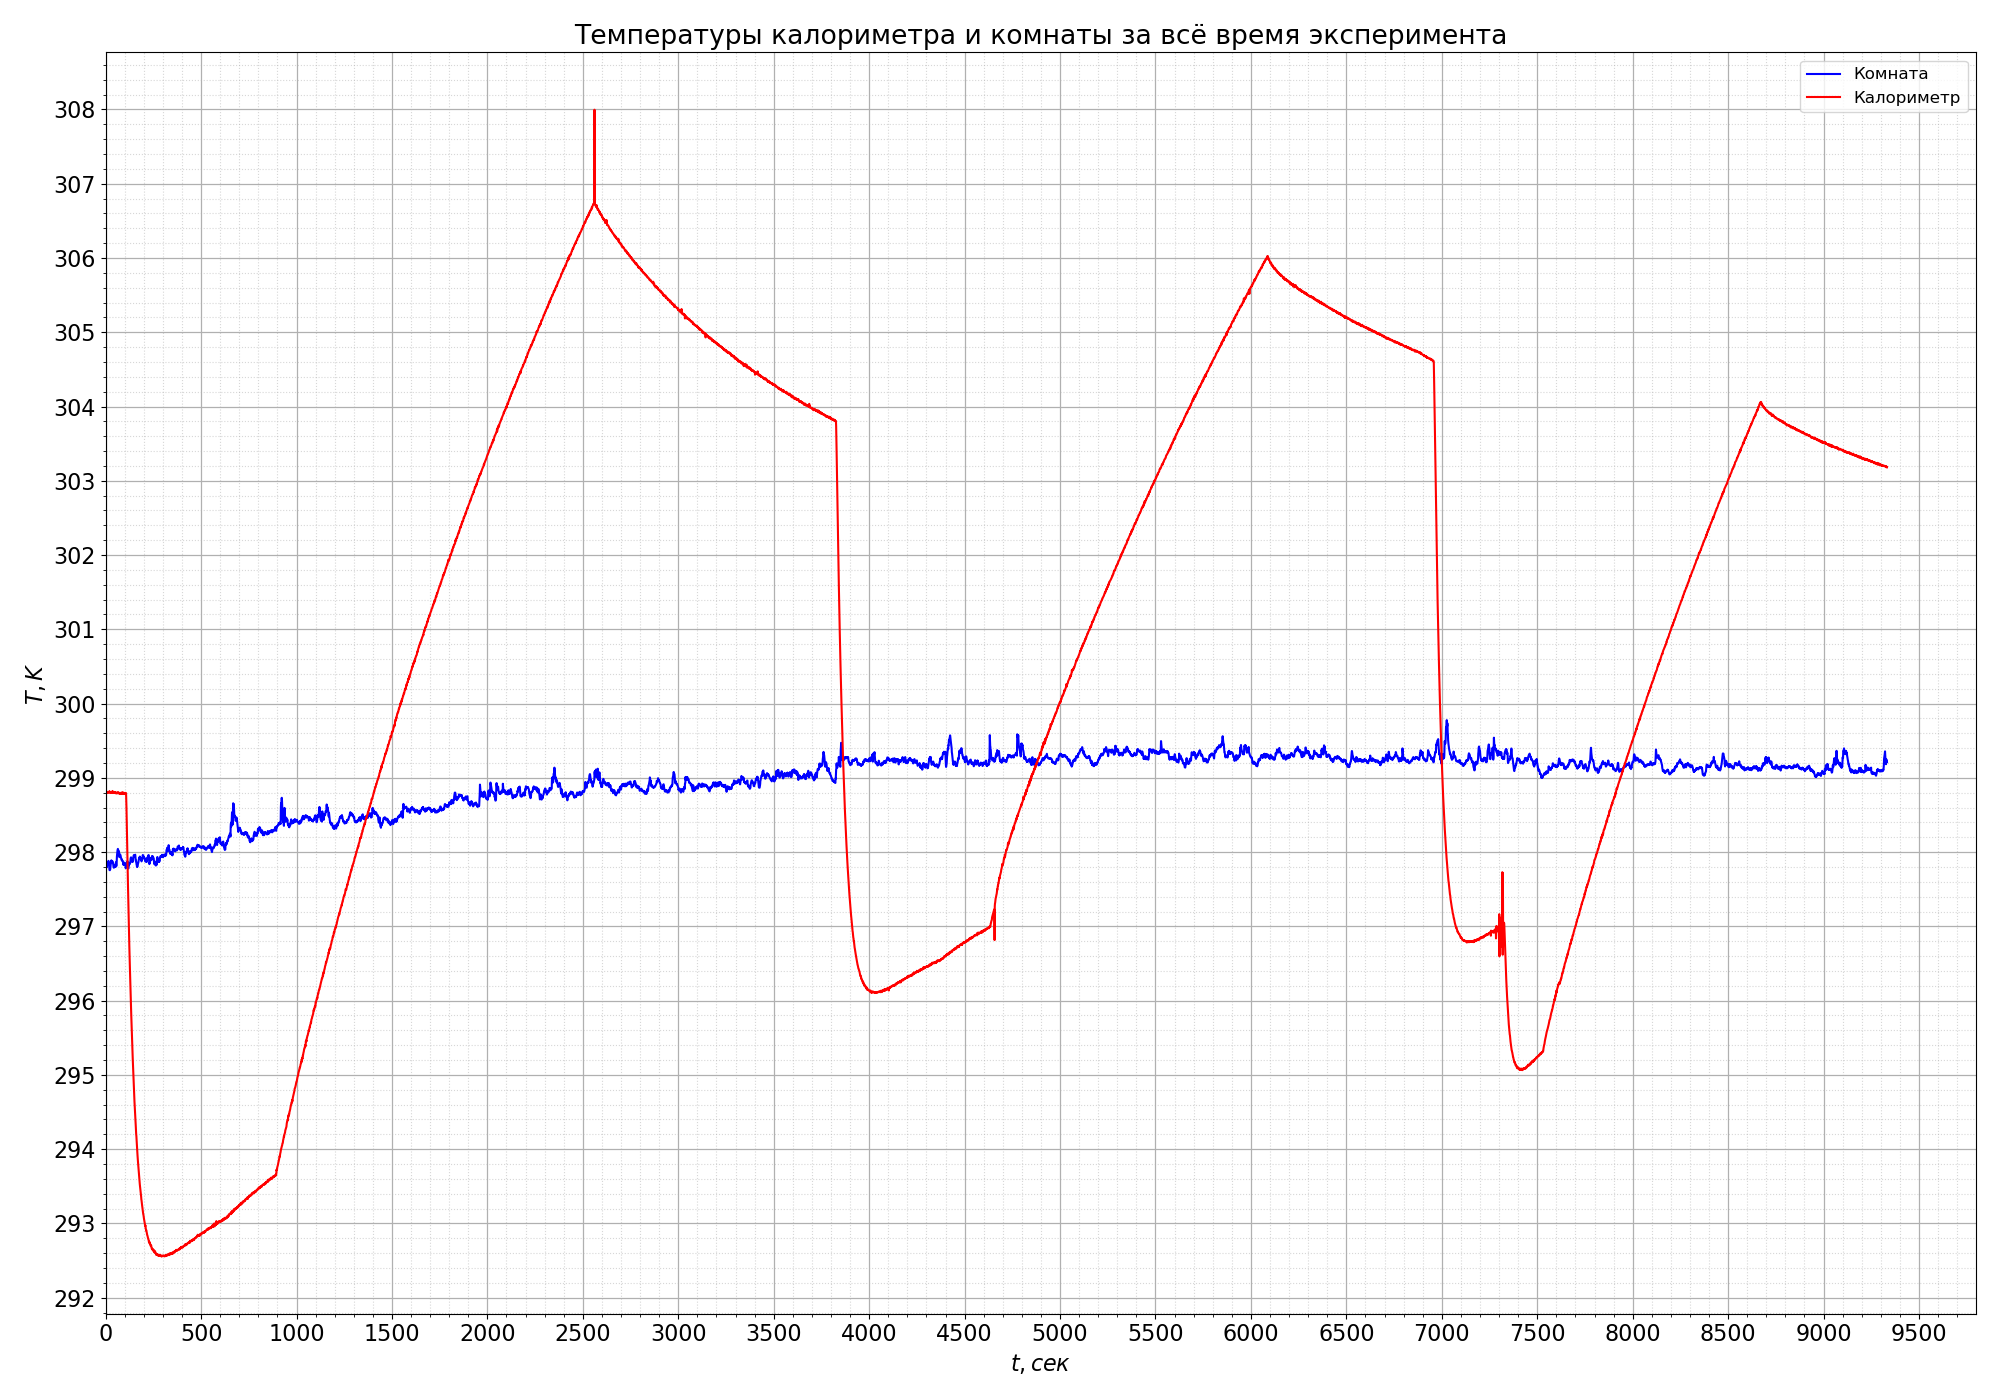
\includegraphics[angle=90,width=0.95\textwidth]{"img/graph_all.png"}
            \caption{Температуры калориметра и комнаты за всё время эксперимента}
            \label{plot:all}
        \end{figure}

\end{document}
